\setcounter{chapter}{1}
%*******************************START Background **********************************

\chapter{Background and Relevant Literature}\label{sec:MAS}

In this chapter, we briefly review web services, then we introduce the concept of communities of web services, their architecture and applications and the benefits of forming communities. Then we discuss the cooperative game theory concepts used throughout our research work. Finally, we discuss the relevant related work on web service communities and games in service oriented computing literature.

    \section{Community of Web Services}\label{sec:CommunityWS}
    In this section, we discuss the concept of communities of web services, and we discuss the architecture and operations of community members.

        \subsection{Web Services}\label{sec:CWSWebServices}
        Over the past years, online services have become part of standard daily life of people around the globe. Many applications these days rely on
        web services from different providers to function. Most modern computer applications, specially
        mobile and tablet applications which have limited storage and processing power
        are merely just an interface aggregating different information from online service providers.
        Examples are vast, weather forecasting, ticket selling, local maps and places search, shopping apps, almost all rely on
        robust web service providers.

        The World Wide Web Consortium (W3C) defines web services as follows: "software
        system designed to support interpretable machine-to-machine interaction over a network.
        It has an interface described in a machine-processable format (specifically WSDL). Other
        systems interact with the web service in a manner prescribed by its description using
        SOAP messages, typically conveyed using HTTP with XML serialization in conjunction
        with other Web-related standards". When developers declare a new web service, it will
        be discovered based on its description that fully describes the service. Developers also
        have to declare a public interface and a readable documentation to help other developers
        when integrating different services \cite{w3cwsdl}. Nowadays Web API standards which do not
        require XML-based web service protocols like SOAP and WSDL are also emerging. They are also called
        REST (representational state transfer) services which are moving towards simpler communication protocols.
        They are not restricted to XML formats, recently JSON, a human readable and simpler format is becoming popular among online service providers.

        We are not going to delve into engineering details of online web service implementation and its protocols in this proposal.
        We consider the service, web services provide as a request-response operation, where they receive a message specifying a question,
        based on this message they generate a response, satisfying end users' need. Service providers usually charge end users for services they provide,
        gaining profit in the process. For example Google has listed their pricing and plans for wide range of services they provide
        on their web service console page\footnote{https://code.google.com/apis/console}.

        In our research work, we abstract web services as rational entities\footnote{The term
        rational is used here in the sense that web services are utility
        maximizers} providing services to end users. They aim to maximize
        their individual income by receiving enough requests from end
        users. In order to increase their revenue, web services seek for
        more tasks if they have the capacity and throughput to do so. Web
        services can join communities to have better efficiency by
        collaborating with others, to have access to higher market share,
        and to have opportunity of receiving a bigger task pool from end
        users. Also the high reliance on web services, has increased quality expectations from end users.
        Communities of web services can provide higher performance, reliability, fail recovery for end users.

        \subsection{Web Service Communities}\label{sec:CWSDefinition}
        Community in dictionary definition refers to "the condition of sharing or having certain attitudes and interests in common" or "a group of people living in the same place or having a particular characteristic in common". In \cite{DBLP:journals/internet/BenatallahSD03, Zeng:2003:QDW:775152.775211} introduce community of web services as collection of cooperative web services with a common service and functionality but different QoS metrics. Therefore $communities$ are differentiated from $composition$ type of web service cooperation in which web services with different functionalities work together to generate a new service provider with composite functionality.


        Maamar et al. initially in \cite{conf/webist/MaamarLBTS07} and then comprehensively in \cite{DBLP:journals/ijebr/MaamarSTBB09} proposed the an architecture
        utilizing \emph{Contract-Net} protocol for engineering community of web services.
        This architecture has been further developed in \cite{conf/IEEEscc/BenharrefSBB11, conf/IEEEscc/KhosravifarBMMT10, conf/aina/LimTM11, CSTintercommunity}.
        Community of web services have two major roles for members of a community, the master and slave web service.
        Master web services lead communities and are responsible for community and membership management of the community, they try to invite and and convince web services to join the
        community. They can attract new web services to their communities by awarding them more payoff. They also can eject some web services from the community improving the
        community and individual member satisfaction, and overall community reputation.

        \begin{figure}
            \begin{center}
            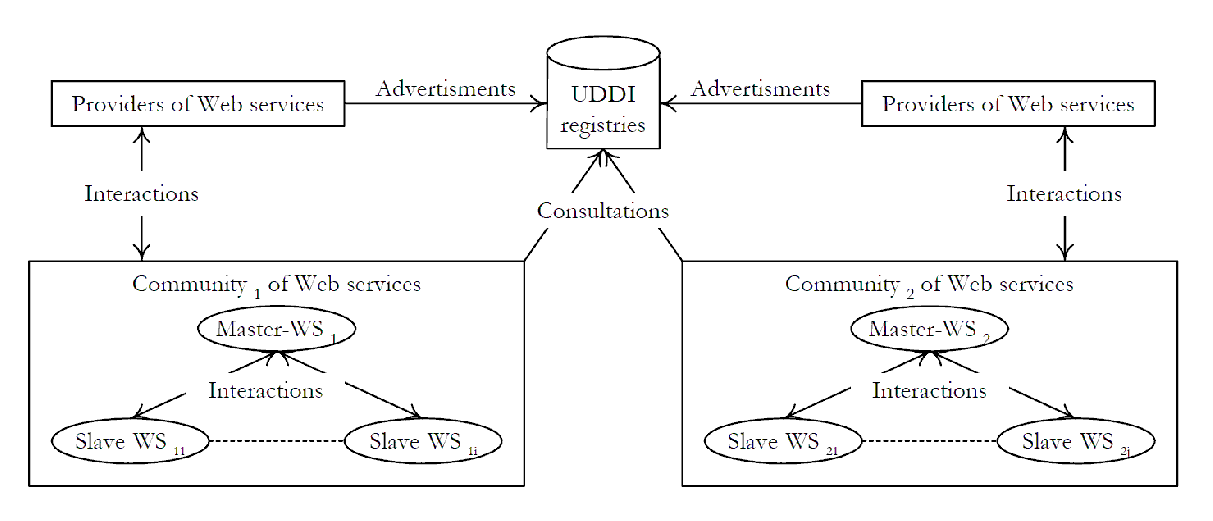
\includegraphics[width=16cm]{Figures/wsarch.eps}\label{wsarch}
            \caption{Communities of Web Services Architecture as Proposed in \cite{DBLP:journals/ijebr/MaamarSTBB09}}
            \end{center}
        \end{figure}

        Figure \ref{wsarch} depicts the basic architecture of communities of web services. The main components of the architecture are: 1) the providers of web services,
        2) UDDI registries and 3) communities of web services. Communities abstract the same model of defining, announcing and invoking of web services. They also adopt the same protocols that standard web services use with UDDI registries. UDDI is a platform-independent XML based registry list which facilitates worldwide web service discovery.

        The master web service is responsible with communication with web service providers and discovery registries. It it responsible for task distribution, web service selection,
        community management, maintaining a healthy set of web services satisfying end users requests with high QoS. In communities, the masters web services can be
        dedicated web services playing the master role during the entire time of being in the community. This master web service is independently developed and never
        participates in any composition. The master web services can also be chosen out of normal web services already inside the community \cite{DBLP:journals/ijebr/MaamarSTBB09}.


    \section{Cooperative Game Theory in Multi-agent Systems}\label{sec:CGTMS}

        \subsection{Cooperative Game Thoery}\label{sec:BRWS}

        \subsection{Motivating Example}\label{sec:CWSDefinition}

        An example which has closely resembles our community service model is the \emph{Single landowner and landless workers} example.
        This example was introduced in \cite{GVK369342747} and represents the \emph{landowner} entity which is providing jobs and \emph{landless workers} who cannot do anything by themselves and need to work with a landowner to gain some income.

        In this game, land is owned by a single person, the \emph{landowner}. We refer to the other people as \emph{workers}. In this case we have a game there the set of players are the landowner and the $m$ workers, possible actions for coalitions with only workers would be distributing the zero output for all where no member receives any output. The set of actions of a coalition $S$ consisting of the landowner and $k$ workers would be the set of all $S$-allocations of the output $f(k+1)$ among the members of $S$. The preference of each player would be the amount of out she obtains.

        \subsection{Cooperative Games in Service Oriented Computing}\label{sec:CWSArchitecture}

        \subsection{Representation and Complexity issues}\label{sec:CWSArchitecture}

    \section{Related Work}\label{sec:BRRelatedWork}

        One of the first contributions in which web service community was introduced was in \cite{Zeng:2003:QDW:775152.775211}. They defined web service community as collection of web services providing same functionality however with different quality metrics.

        Medjahed and Boubuettaya \cite{journals/dpd/MedjahedB05} have proposed a framework and a community builder mechanism which uses semantic analysis, providing an ontological organization of web services having same domain of interest. The community builder would suggest web services having similar operations with any community to join the community, or form their own communities in case the semantic analysis cannot find any community with close enough operations and service types.

        Most of the recent work on communities of services are either
        user-centric and focus on user satisfaction
        \cite{Chun02user-centricperformance} or system-centric and focus
        on the whole system throughput, performance and utilization. There
        are many contributions in distributed, grid, cluster and cloud
        services which are system-centric. However, in real world
        environments and applications, both users and service providers
        are self-interested agents, aiming to maximize their own profit.
        In those environments, both parties (users and services) will
        collaborate as long as they are getting more benefits and payoff.

        In this direction, recently \cite{DBLP:conf/IEEEscc/LimTMB12,
        DBLP:conf/IEEEscc/KhosravifarABT11, 10.1109/TSC.2012.12} proposed mechanisms to help
        users and services to maximize their gain. A two-player
        non-cooperative game between web services and community master was
        introduced in \cite{DBLP:conf/IEEEscc/KhosravifarABT11}. In this
        game-theoretic model, the strategies available to a web service
        when facing a new community are requesting to join the community,
        accepting the master's invitation to join the community, or
        refusing the invitation to join. The set of strategies for
        communities are inviting the web service or refusing the web
        service's join request. Based on their capacity, market share and
        reputation, the two players have different set of utilities over
        the strategy profiles of the game. The main limits of this game
        model are: 1) its consideration of only three quality parameters,
        while the other factors are simply ignored; and 2) the
        non-consideration of the web services already residing within the
        community. The game is only between the community master and the
        new web service, and the inputs from all the other members are
        simply ignored. The consideration of those inputs is a significant
        issue as existing web services can lose utility or payoff because
        of the new member, which can results in an unhealthy and unstable
        group. The problem comes from the fact that the existing members
        should collaborate with the new web services, so probably their
        performance as a group can suffer. Existing members may even
        deviate and try to join other communities if they are unsatisfied.
        Those considerations of forming stable and efficient coalitions
        are the main contributions of our paper.

        In \cite{DBLP:conf/IEEEscc/LimTMB12}, a 3-way satisfaction approach
        for selecting web services has been proposed. In this approach,
        the authors proposed a web service selection process that the
        community masters can use. The approach considers the efficiency
        of all the three involved parties, namely users, web services and
        communities. In this work, it is shown how the gains of these
        parties are coupled together using a linear optimization process.
        However, the optimization problem in this solution tends to
        optimize some parameters considering all web services regardless
        of their efficiency and contribution to the community's welfare.
        Moreover, there are no clear thresholds for accepting or rejecting
        new web services. The solution of the optimization problem could,
        for instance, suggest web services already residing within the
        community to increase or decrease their capacity to cover up the
        weakness of other parties in the system. However, a high
        performing web service could deviate anytime it finds itself
        unsatisfied within the community instead of adjusting its service
        parameters.

        In \cite{10.1109/TSC.2012.12}, a cooperative scheme among autonomous
        web services based on coalitional game theory has been introduced. They have proposed an algorithm to
        reach individually stable coalition partition for web services in order to
        maximize their efficiency. The communities choose new web services on the promise
        that it would benefit the community without decreasing any other web service's
        income. In their model, the worth of community is evaluated with high emphasis on
        availability metric and considering price and cost values only. The community structure is based on a coordination chain,
        where a web service is assigned as a \emph{primary} web service and the community task destribution
        method, will initially invoke the primary web service and only if the primary web service is unavailable
        will invoke the next backup web services as they are ordered in the coordination chain. However in cooperative models, it is preferred to
        have a real and active cooperative activity engaging all agents to perform the tasks more efficiently. Especially nowadays
        with recent advancement in cloud and hardware infrastructures availability is becoming less of an issue. So the backup web services
        in their model have a very low chance of getting jobs, especially the ones further in chain, which is huge waste of web services
        capabilities.

Cooperative game theory provides a set of mathematical and optimization tools for multi-agent environments. These tools have been utilized in communication networks and service oriented computing literature, where nodes as rational agents try to reason strategically and maximise their benefit.





%*******************************End Background **********************************
